\documentclass[8pt]{beamer}  
\usetheme{Madrid}
\usecolortheme{beetle}
\usepackage[orientation=landscape,size=custom,width=16,height=9,scale=0.5,debug]{beamerposter} 
\usepackage{xcolor}
\usepackage{amsmath}
\setbeamercolor{background canvas}{bg=blue!15!red!35!green!82!black}
\setbeamercolor{normal text}{fg=white}
\usebeamercolor[fg]{normal text}
\setbeamercolor{frametitle}{fg=yellow}
\usefonttheme[onlymath]{serif}
\newcommand{\pauseditem}{\pause \item[]}


\newcommand{\Tup}[0]{\mathbf S}
\newcommand{\bh}[0]{\mathbf h}
\newcommand{\ba}{\mathbf a}
\newcommand{\bb}{\mathbf b}
\newcommand{\bc}{\mathbf c}
\newcommand{\sbbbb}[0]{\bsigma_{\mathbf b}}
\newcommand{\scccc}[0]{\bsigma_{\mathbf c}}
\newcommand{\bsigma}{\mathbf \sigma}
\newcommand{\sh}[0]{\bsigma_{\mathbf h}}
\newcommand{\sa}[0]{\bsigma_{\mathbf a}}


\title{A New Equation for Period Vectors of Crystals under External Stress and Temperature in Statistical Physics}

\subtitle{ {\color{yellow} Mechanical Equilibrium Condition and Equation of State}}

\author{Gang Liu}

\institute
{ gl.cell@outlook.com \\
https://github.com/LiuGangKingston \\
http://www.linkedin.com/in/liuganglinkedin \\
https://doi.org/10.1140/epjp/s13360-020-01010-6 \\
Independent Researcher, Kingston, Ontario, Canada
}

\date {June 29th, 2021}


\AtBeginSection[]
{
  \begin{frame}
    \frametitle{Table of Contents}
    \tableofcontents[currentsection]
  \end{frame}
}




\begin{document}
\frame{\titlepage}

\begin{frame}
\frametitle{Table of Contents}
\tableofcontents
\end{frame}




\section{The publication}

\begin{frame}{Article by EPJP as \# 48, 2021 (136)}

{\centering \vspace{-.2cm} {https://doi.org/10.1140/epjp/s13360-020-01010-6} }

\begin{columns}
      \vspace{1cm} \hspace{.0cm}
      \column{0.5\textwidth}
      \begin{figure} 
          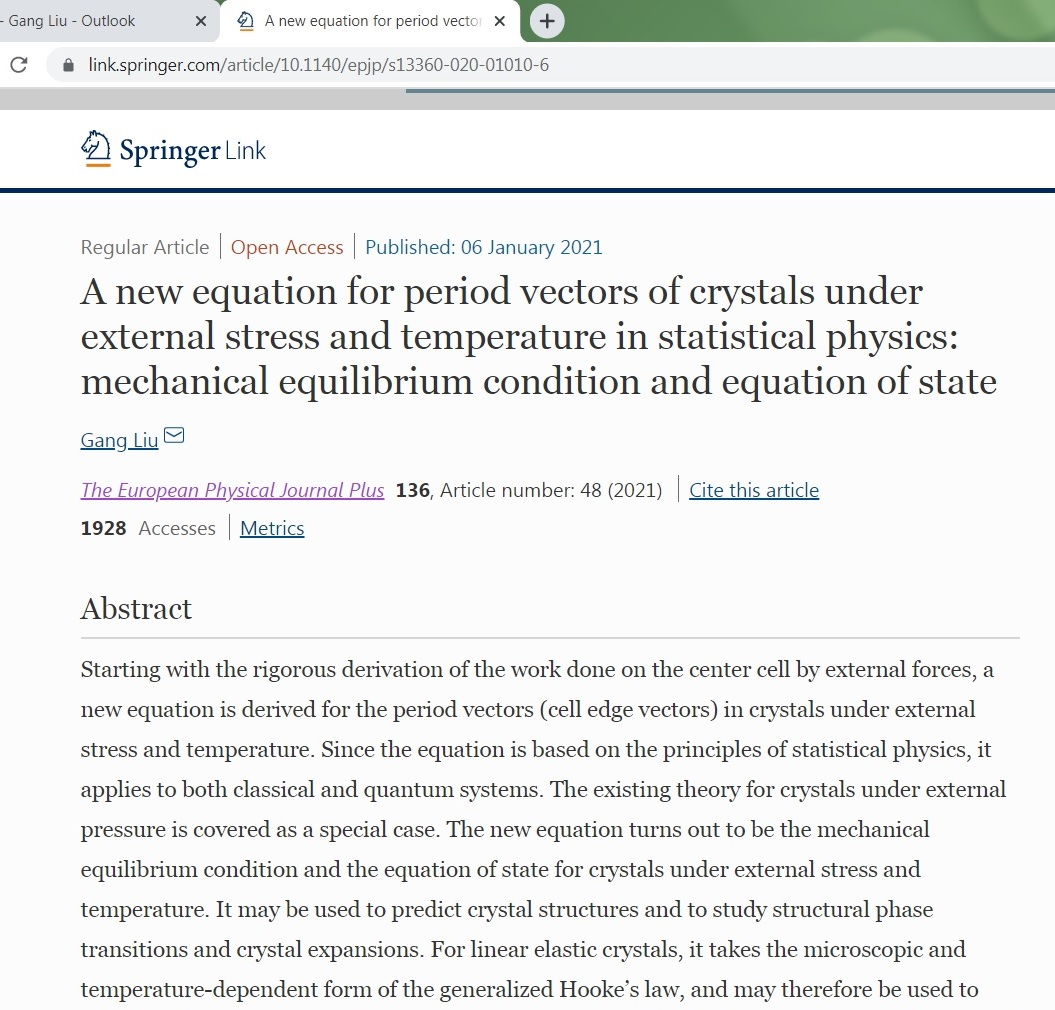
\includegraphics[width=1.\textwidth]{./w02.jpg}
      \end{figure} 
       
      \column{0.5\textwidth}
      \begin{figure} 
          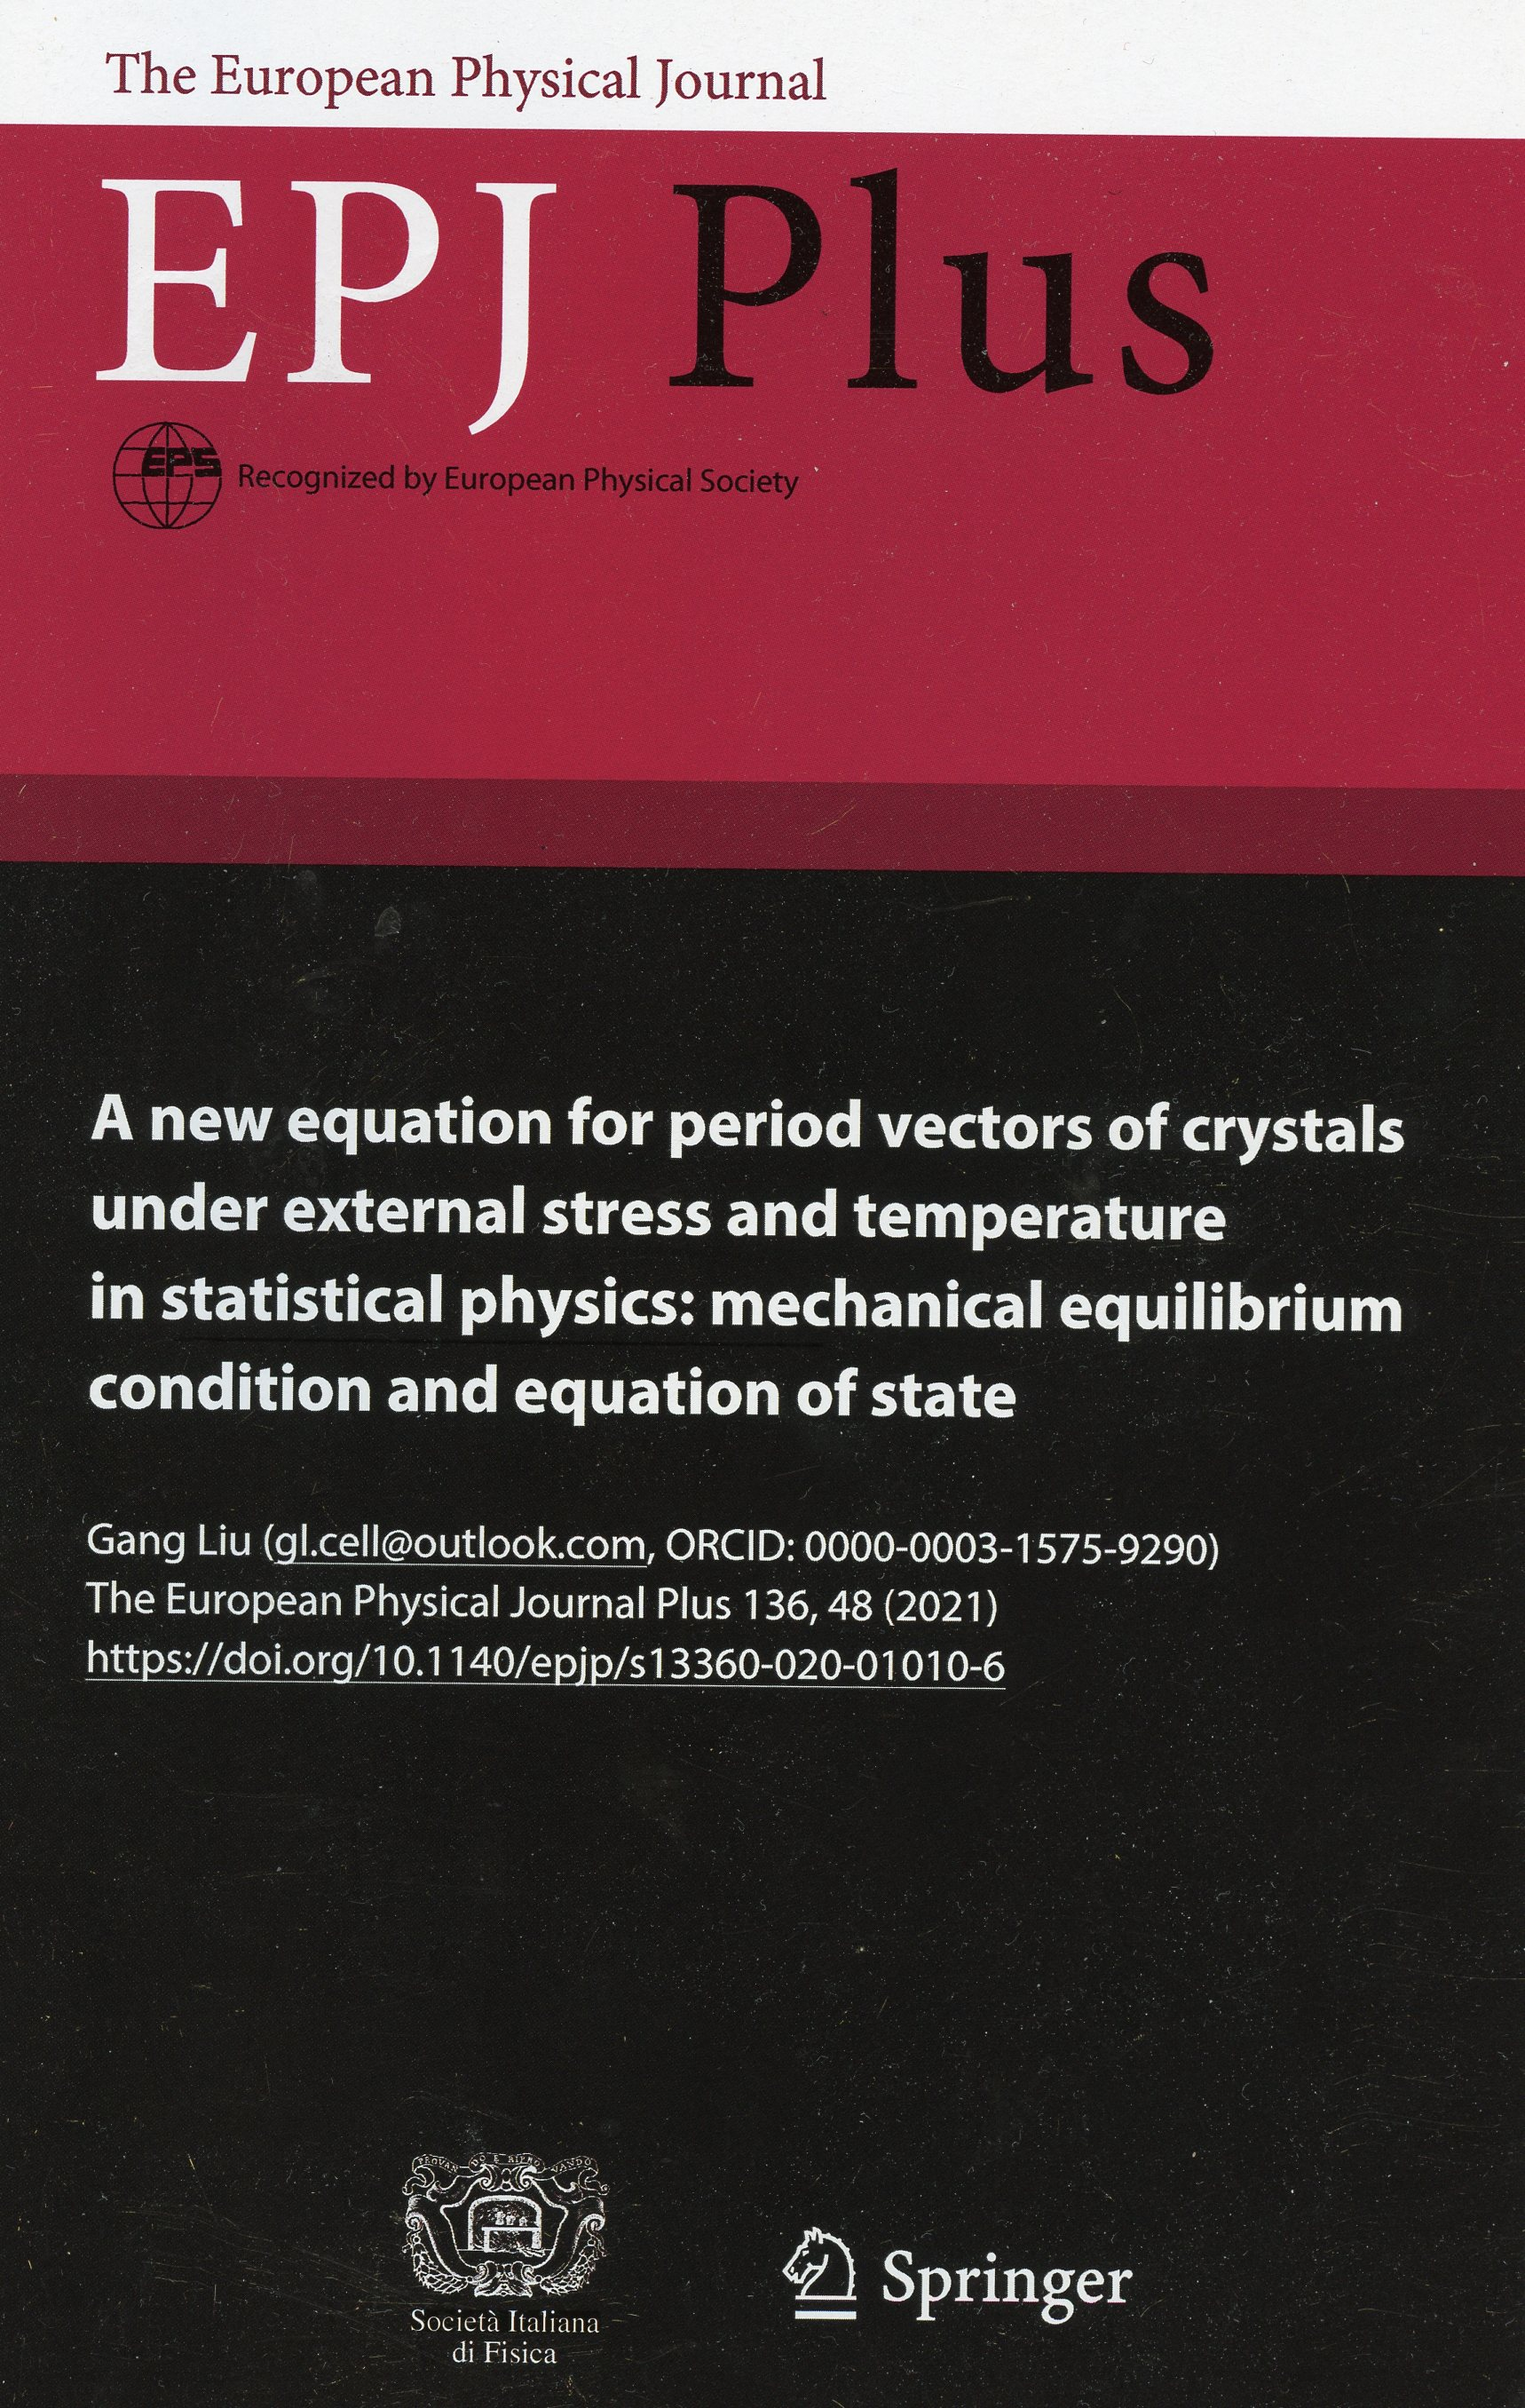
\includegraphics[width=.6\textwidth]{./img264.jpg}
      \end{figure}
\end{columns}
\end{frame}




\section{The derived equation }

\begin{frame}{The work done on the center cell by the external stress $\Tup$}
\vspace{-.5cm}
\begin{equation}
      dW =(\Tup \cdot \sa) \cdot d\ba + (\Tup \cdot \sbbbb) \cdot d\bb + (\Tup \cdot \scccc) \cdot d\bc  \label{sss080}
\end{equation}
\vspace{-1.5cm}
      \begin{figure} 
          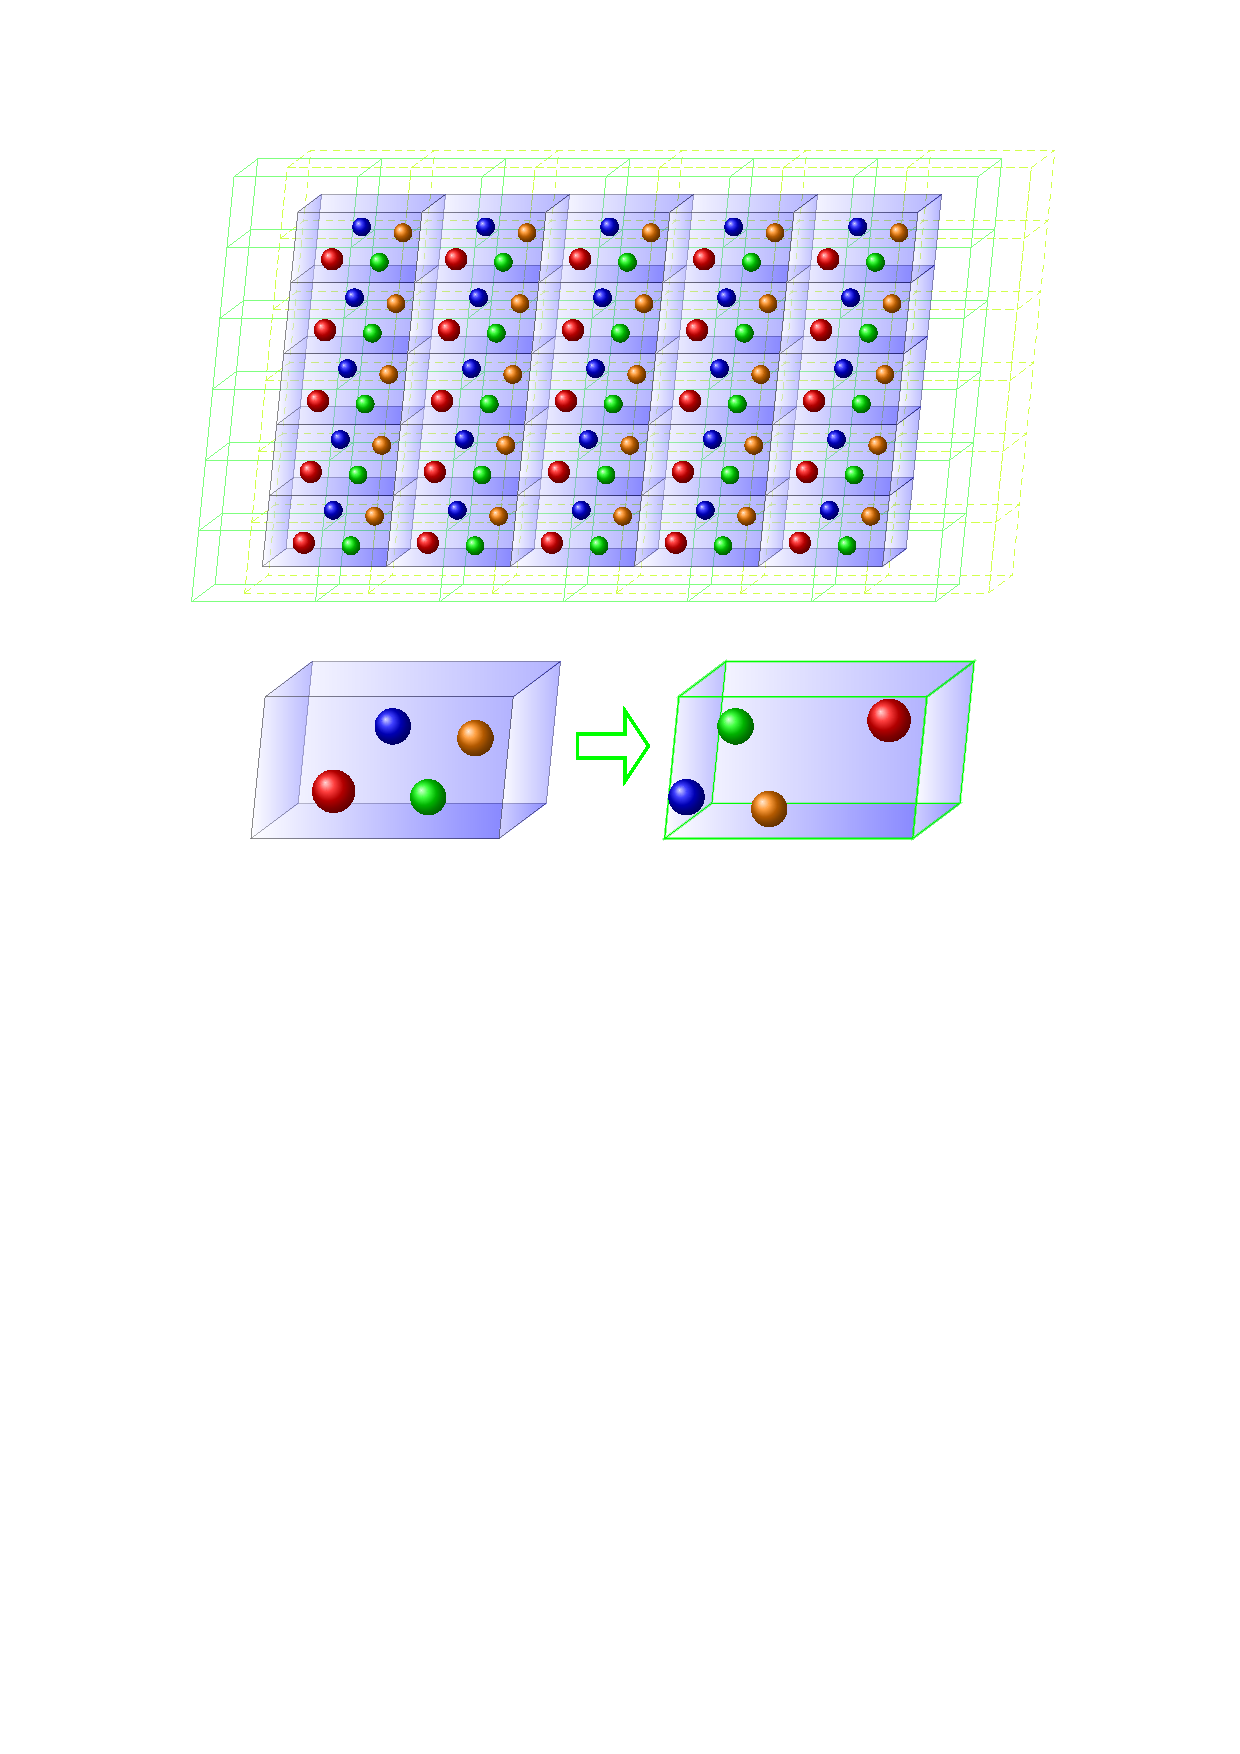
\includegraphics[width=.8\textwidth]{./translated_cells_by_tikz.pdf}
      \end{figure}
\end{frame}


\begin{frame}{Then based on the principles of statistical physics, the new equation determining the period vectors ($\ba, \bb, \bc$) for crystals under external stress $\Tup$ and temperature $T$: }

\vspace{-1.7cm}{\LARGE  \color{white}{
\begin{equation}
       \Tup \cdot \sh=-\frac {1}{\beta} \frac {\partial \ln Z}{\partial \bh} \ \ \ (\bh=\ba, \bb, \bc) ,
       \label{sss100}
\end{equation}
}}

where $\beta=1/(kT)$, and $k$ and $Z$ are the Boltzmann constant and the system partition function. The cell surface vectors are $\sa=\bb \times \bc$, $\sbbbb=\bc \times \ba$, and $\scccc=\ba \times \bb$.
\end{frame}




\section{The net force on the right by the left in the example}

\begin{frame}
{The net force by the left half on the right half of the one-dimensional crystal}
\vspace{-1.2cm}
\begin{itemize}
    \begin{eqnarray}
           F_{L\rightarrow R} \left( a \right) 
           &=&  - \frac{d}{da} E_p^{(L-J)} \left( a \right) \\
           \pauseditem &=& \frac 12 \sum_{ j=-\infty} ^{\infty (j \neq 0)} 
                           j f^{(L-J)} \left(  j a \right) \\
           \pauseditem &=& \sum_{ j=1} ^\infty \frac{4 \epsilon}{a}  
                           \left [ { 12 \left ( \frac{\lambda} 
                           { j a} \right ) }^{12} - 
                           { 6 \left ( \frac{\lambda} { j a} \right ) }^{6} 
                           \right ] 
    \end{eqnarray}
\end{itemize}
\end{frame}




\end{document}